\chapter{Problems and Procedures}\label{ch:problems}\label{ch:procedures}

\chapquotew{A great discovery solves a great problem, but there is a grain of discovery in the solution of any problem. Your problem may be modest, but if it challenges your curiosity and brings into play your inventive faculties, and if you solve it by your own means, you may experience the tension and enjoy the triumph of discovery.}{George P\'olya, \emph{How to Solve It}}{11.5cm}\index{people}{P\'olya, George}

%% room for another short quote [chapter 9] \chapquotew{If you keep proving stuff that others have done, getting confidence, increasing the complexities of your solutions --- for the fun of it --- then one day you'll turn around and discover that nobody actually did that one! And that's the way to become a computer scientist.}{Richard Feynman, \emph{Lectures on Computation}}{10.2cm}\index{people}{Feynman, Richard}

\begin{schemeregion}

Computers are tools for performing computations to solve problems.  In this chapter, we consider what it means to solve a problem and explore some strategies for constructing procedures that solve problems.

\section{Solving Problems}

Traditionally, a problem is an obstacle to overcome or some question to answer.  Once the question is answered or the obstacle circumvented, the problem is solved and we can declare victory and move on to the next one.  

When we talk about writing programs to solve problems, though, we have a larger goal.  We don't just want to solve \emph{one} instance of a problem, we want an algorithm that can solve \emph{all} instances of a problem.  A \definition{problem} is defined by its inputs and the desired property of the output.  Recall from Chapter~\ref{ch:intro}, that a procedure is a precise description of a process and a procedure is guaranteed to always finish is called an \emph{algorithm}.\index{general}{algorithm}  The name algorithm is a Latinization of the name of the Persian mathematician and scientist, Muhammad ibn M\={u}s\={a} al-Khw\={a}rizm\={\i}, who published a book in 825 on calculation with Hindu numerals.  \cut{Al-Khw\={a}rizm\={\i} was also the responsible for defining algebra.  } %http://en.wikipedia.org/wiki/Muhammad_ibn_M%C5%ABs%C4%81_al-Khw%C4%81rizm%C4%AB
%\sidepicture{0.65}{images/Khwarizmii.jpg}{al-Khw\={a}rizm\={\i}}{}% public domain
Although the name algorithm was adopted after al-Khw\={a}rizm\={\i}'s book, algorithms go back much further than that.  The ancient Babylonians had algorithms for finding square roots more than 3500 years ago (see Exploration~\ref{exploration:sqrt}).  \cut{~\cite{Knuth1972}}

For example, we don't just want to find the best route between New York and Washington, we want an algorithm that takes as inputs the map, start location, and end location, and outputs the best route.  There are infinitely many possible inputs that each specify different instances of the problem; a general solution to the problem is a procedure that finds the best route for all possible inputs.\footnote{Actually finding a general algorithm that does without needing to essentially try all possible routes is a challenging and interesting problem, for which no efficient solution is known.  Finding one (or proving no fast algorithm exists) would resolve the most important open problem in computer science!}

%% should define procedure also!
To define a procedure that can solve a problem, we need to define a procedure that takes inputs describing the problem instance and produces a different information process depending on the actual values of its inputs.  A procedure takes zero or more inputs, and produces one output or no outputs\footnote{Although procedures can produce more than one output, we limit our discussion here to procedures that produce no more than one output.  In the next chapter, we introduce ways to construct complex data, so any number of output values can be packaged into a single output.}, as shown in Figure~\ref{fig:procedure}.

\begin{figure}[!ht]
\begin{center}
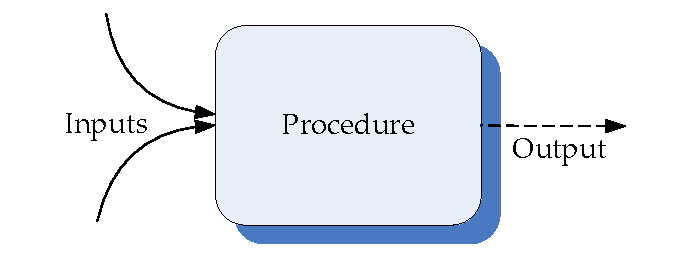
\includegraphics[height=1.0in]{figures/procedure.pdf}
\caption{A procedure maps inputs to an output.\label{fig:procedure}}
\end{center}
\end{figure}

Our goal in solving a problem is to devise a procedure that takes inputs that define a problem instance, and produces as output the solution to that problem instance.  The procedure should be an algorithm --- this means every application of the procedure must eventually finish evaluating and produce an output value.  

%Some programs are intended to provide a service rather than just one output.  For example, a web server is a program that is intended to run forever.  It keeps running, waiting for and responding to new requests.  Even programs that are services, however, involve algorithms.  Each individual web request is a problem, and the server program should respond to it with a particular output (sending the requested page) within a reasonable amount of time.

There is no magic wand for solving problems.  But, most problem solving involves breaking problems you do not yet know how to solve into simpler and simpler problems until you find problems simple enough that you already know how to solve them.  The creative challenge is to find the simpler subproblems that can be combined to solve the original problem.  This approach of solving problems by breaking them into simpler parts is known as \definition{divide-and-conquer}.

The following sections describe a two key forms of divide-and-conquer problem solving: composition and recursive problem solving.  We will use these same problem-solving techniques in different forms throughout this book.

%\marginquote{The central purpose of the University of Virginia is to enrich the mind by stimulating and sustaining a spirit of free inquiry directed to understanding the nature of the universe and the role of mankind in it. Activities designed to quicken, discipline, and enlarge the intellectual and creative capacities, as well as the aesthetic and ethical awareness, of the members of the University and to record, preserve, and disseminate the results of intellectual discovery and creative endeavor serve this purpose.}{\emph{Institutional Purpose of The University of Virginia}, Board of Visitors Manual (adopted in 1985)}

\section{Composing Procedures}\label{sec:compose}\index{general}{composition}

One way to divide a problem is to split it into steps where the output of the first step is the input to the second step, and the output of the second step is the solution to the problem.  Each step can be defined by one procedure, and the two procedures can be combined to create one procedure that solves the problem.  

Figure~\ref{fig:composition} shows a composition of two functions, \scheme|f| and \scheme|g|.  The output of \emph{f} is used as the input to \emph{g}.  

\begin{figure}[!ht]
\begin{center}
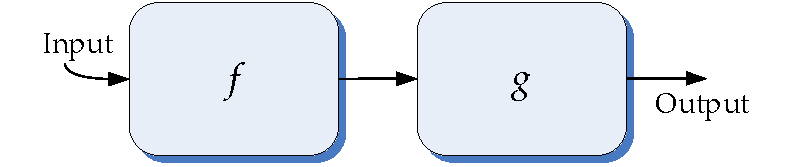
\includegraphics[height=0.8in]{figures/composition.pdf}
\caption{Composition.\label{fig:composition}}
\end{center}
\end{figure}

We can express this composition with the Scheme expression \scheme|(g (f x))| where \scheme|x| is the input.  The written order appears to be reversed from the picture in  Figure~\ref{fig:composition}.  This is because we apply a procedure to the values of its subexpressions: the values of the inner subexpressions must be computed first, and then used as the inputs to the outer applications.  So, the inner subexpression \scheme|(f x)| is evaluated first since the evaluation rule for the outer application expression is to first evaluate all the subexpressions.  

To define a procedure that implements the composed procedure we make \scheme|x| a parameter:
\begin{schemedisplay}
(define fog (lambda (x) (g (f x))))
\end{schemedisplay}
This defines \scheme{fog} as a procedure that takes one input and produces as output the composition of \scheme|f| and \scheme|g| applied to the input parameter.  This works for any two procedures that both take a single input parameter.

We can compose the \scheme|square| and \scheme|cube| procedures from Chapter~\ref{ch:programming}:
\begin{schemedisplay}
(define sixth-power (lambda (x) (cube (square x))))
\end{schemedisplay}
Then, \scheme|(sixth-power 2)| evaluates to \schemeresult|64|.  

\subsection{Procedures as Inputs and Outputs}\label{sec:fcompose}

All the procedure inputs and outputs we have seen so far have been numbers.  The subexpressions of an application can be any expression including a procedure.  A \definition{higher-order procedure} is a procedure that takes other procedures as inputs or that produces a procedure as its output.  Higher-order procedures give us the ability to write procedures that behave differently based on the procedures that are passed in as inputs.  

We can create a generic composition procedure by making \scheme|f| and \scheme|g| parameters:
\begin{schemedisplay}
(define fog (lambda (f g x) (g (f x))))
\end{schemedisplay}
The \scheme|fog| procedure takes three parameters.  The first two are both procedures that take one input.  The third parameter is a value that can be the input to the first procedure.

For example, \scheme|(fog square cube 2)| evaluates to \tb{\schemeresult|64|}, and  \scheme|(fog (lambda (x) (+ x 1)) square 2)| evaluates to \tb{\schemeresult{9}}.  In the second example, the first parameter is the procedure produced by the lambda expression \scheme|(lambda (x) (+ x 1))|.  This procedure takes a number as input and produces as output that number plus one.  We use a definition to name this procedure \scheme|inc| (short for increment):
\index{general}{inc}
\begin{schemedisplay}
(define inc (lambda (x) (+ x 1)))
\end{schemedisplay}

A more useful composition procedure would separate the input value, \scheme|x|, from the composition.  The \scheme|fcompose| procedure takes two procedures as inputs and produces as output a procedure that is their composition:\footnote{We name our composition procedure \scheme|fcompose| to avoid collision with the built-in \scheme|compose| procedure that behaves similarly.}
\index{general}{fcompose}\index{general}{compose}
\begin{schemedisplay}
(define fcompose
   (lambda (f g) (lambda (x) (g (f x)))))
\end{schemedisplay}
The body of the \scheme|fcompose| procedure is a lambda expression that makes a procedure.  Hence, the result of applying \scheme|fcompose| to two procedures is not a simple value, but a procedure.  The resulting procedure can then be applied to a value.

Here are some examples using \scheme|fcompose|:
\begin{code}
\scheme|> (fcompose inc inc)|\\
\tb{\schemeresult|#<procedure>|}\\
\scheme|> ((fcompose inc inc) 1)|\\
\tb{\schemeresult|3|}\\
%\scheme|> (define sixth-power (fcompose square cube))|\\
%\scheme|> (sixth-power 3)|\\
%\tb{\schemeresult|729|}\\
\scheme|> ((fcompose inc square) 2)|\\
\tb{\schemeresult|9|}\\
\scheme|> ((fcompose square inc) 2)|\\
\tb{\schemeresult|5|}\\
\end{code}
\cut{Note that the order in which procedures are composed matters.  For example, \scheme|(((fcompose inc square) 2)|) evaluates to \schemeresult|9| since the input is incremented first, then squared; but, \scheme|((fcompose square inc) 2)| evaluates to \schemeresult|5|.}

\beforeex
\begin{exercise}
For each expression, give the value to which the expression evaluates.  Assume \scheme|fcompose| and \scheme|inc| are defined as above.
\begin{subexerciselist}
\item \scheme|((fcompose square square) 3)|
\solution{The application expression \scheme|(fcompose square square)| evaluates to a procedure that composes square with square (that is, it multiples its input by itself four times).  Hence, applying this procedure to \scheme|3| evaluates to \scheme|81|.}
\item \scheme|(fcompose (lambda (x) (* x 2)) (lambda (x) (/ x 2)))|
\solution{This evaluates to an identity procedure for number inputs.  It produces a procedure that takes a number as its input, and applies a procedure that multiplies by \scheme|2| to the result of a procedure that divides the input number by \scheme|2|.}  
\item \scheme|((fcompose (lambda (x) (* x 2)) (lambda (x) (/ x 2))) 1120)|
\solution{This applies the identity procedure from the previous part to \scheme|1120|, so the result is \schemeresult|1120|.}
\item \scheme|((fcompose (fcompose inc inc) inc) 2)|
\solution{The inner application expression, \scheme|(fcompose inc inc)|, evaluates to a procedure that takes a number as its input and outputs the result of incrementing it twice (that is, adding \scheme|2|).  The next application expression, \scheme|(fcompose (fcompose inc inc) inc)|, composes this with another \scheme|inc| procedure, producing a procedure that adds \scheme|3| to its input.  Applying this procedure to \scheme|2| results in the value \schemeresult|5|.}
\end{subexerciselist}
\end{exercise}
\afterex

\beforeex
\begin{exercise}
Suppose we define \scheme|self-compose| as a procedure that composes a procedure with itself:
\begin{schemedisplay}
(define (self-compose f) (fcompose f f))
\end{schemedisplay}
Explain how \scheme|(((fcompose self-compose self-compose) inc) 1)| is evaluated.
\solution{The application expression, \scheme|(fcompose self-compose self-compose)|, produces a procedure that composes \scheme|self-compose| with itself.  Using the substitution evaluation rules and the definition of \scheme|fcompose|, this expression evaluates to
\begin{schemedisplay}
((lambda (f g) (lambda (x) (g (f x)))) self-compose self-compose)
\end{schemedisplay}
which evaluates to \scheme|(lambda (x) (self-compose (self-compose x)))|.  Applying this to \scheme|inc| results in
\scheme|(self-compose (self-compose inc))|.  Substituting the definition of \scheme|self-compose|, we get:
\begin{schemedisplay}
(fcompose (fcompose inc inc) (fcompose inc inc))
\end{schemedisplay}  
Now, we can substitute the definition of \scheme|fcompose| for the outer application to get:
\begin{schemedisplay}
(lambda (x) ((fcompose inc inc) ((fcompose inc inc) x))) 
\end{schemedisplay}
This expression is applied to \scheme|1|, producing \scheme|((fcompose inc inc) ((fcompose inc inc) 1))|.  Next, we substitute the definition of \scheme|fcompose| in the inner application to get:
\begin{schemedisplay}
((fcompose inc inc) (((lambda (f g) (lambda x) (g (f x))) inc inc) 1))
\end{schemedisplay}
Using the application rule, this simplifies to \scheme|((fcompose inc inc) ((lambda (x) (inc (inc x))) 1))|.  Applying again, substituting \scheme|1| for \scheme|x|, we get:
\begin{schemedisplay}
((fcompose inc inc) (inc (inc 1)))
\end{schemedisplay}
After performing the \scheme|inc| applications, this is
\scheme|((fcompose inc inc) 3)|.  The remaining application expressions are evaluated the same way, producing the final value of \schemeresult|5|.}
\end{exercise}
\afterex

\beforeex
\begin{exercise}
Define a procedure \scheme|fcompose3| that takes three procedures as input, and produces as output a procedure that is the composition of the three input procedures.  For example, \scheme|((fcompose3 abs inc square) -5)| should evaluate to \schemeresult|36|.  Define \scheme|fcompose3| two different ways: once without using \scheme|fcompose|, and once using \scheme|fcompose|.
\solution{
Without using \scheme|fcompose|:
\begin{schemedisplay}
(define (fcompose3 f1 f2 f3)
   (lambda (x) (f3 (f2 (f1 x)))))
\end{schemedisplay}
Using \scheme|fcompose|:
\begin{schemedisplay}
(define (fcompose3 f1 f2 f3)
   (fcompose (fcompose f1 f2) f3))
\end{schemedisplay}
}
\end{exercise}
\afterex

\beforeex
\begin{exercise}
The \scheme|fcompose| procedure only works when both input procedures take one input. Define a \scheme|f2compose| procedure that composes two procedures where the first procedure takes two inputs, and the second procedure takes one input.  For example, \scheme|((f2compose + abs) 3 -5)| should evaluate to \scheme|2|.
\solution{
\begin{schemedisplay}
(define (f2compose f g)
	(lambda (x y)
	   (g (f x y))))
\end{schemedisplay}}
\end{exercise}
\afterex

\section{Recursive Problem Solving}

\index{general}{recursive definition|(}In the previous section, we used functional composition to break a problem into two procedures that can be composed to produce the desired output.  A particularly useful variation on this is when we can break a problem into a smaller version of the original problem.  
%When coaches speak of taking things ``one game at a time'' this is what they are doing: breaking the problem of winning a championship into the problem of winning the next game, and the problem of winning the rest of the games.

The goal is to be able to feed the output of one application of the procedure back into the same procedure as its input for the next application, as shown in Figure~\ref{fig:circular}.  

\begin{figure}[!hbt]
\begin{center}
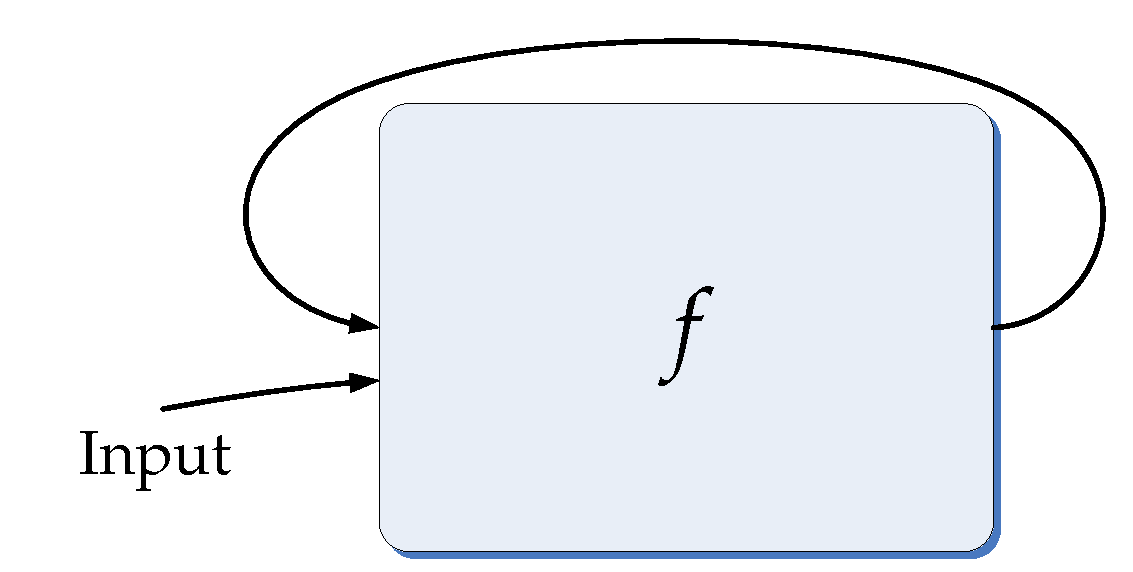
\includegraphics[height=1.0in]{figures/circularcomposition.pdf} 
\caption{Circular Composition.\label{fig:circular}}
\end{center}
\end{figure}

Here's a corresponding Scheme procedure:
\begin{schemedisplay}
(define f (lambda (n) (f n)))
\end{schemedisplay}
Of course, this doesn't work very well!\footnote{Curious readers should try entering this definition into a Scheme interpreter and evaluating \scheme|(f 0)|.  If you get tired of waiting for an output, in DrRacket you can click the \bold{Stop} button in the upper right corner to interrupt the evaluation.}  Every application of \scheme|f| results in another application of \scheme|f| to evaluate.  This never stops --- no output is ever produced and the interpreter will keep evaluating applications of \scheme|f| until it is stopped or runs out of memory.

We need a way to make progress and eventually stop, instead of going around in circles.  To make progress, each subsequent application should have a \emph{smaller} input.  Then, the applications stop when the input to the procedure is simple enough that the output is already known.  The stopping condition is called the \definition{base case}, similarly to the grammar rules in Section~\ref{sec:grammars}.  In our grammar examples, the base case involved replacing the nonterminal with nothing (e.g., \bnfshowrule{MoreDigits}{$\epsilon$}) or with a terminal (e.g., \bnfshowrule{Noun}{\terminal{Alice}}).  In recursive procedures, the base case will provide a solution for some input for which the problem is so simple we already know the answer.  When the input is a number, this is often (but not necessarily) when the input is \scheme|0| or \scheme|1|.

To define a recursive procedure, we use an if expression to test if the input matches the base case input.  If it does, the consequent expression is the known answer for the base case.  Otherwise, the recursive case applies the procedure again but with a smaller input.  That application needs to make progress towards reaching the base case.  This means, the input has to change in a way that gets closer to the base case input.  If the base case is for \scheme|0|, and the original input is a positive number, one way to get closer to the base case input is to subtract \scheme|1| from the input value with each recursive application.

This evaluation spiral is depicted in Figure~\ref{fig:recursion}.  With each subsequent recursive call, the input gets smaller, eventually reaching the base case.  For the base case application, a result is returned to the previous application.  This is passed back up the spiral to produce the final output.  Keeping track of where we are in a recursive evaluation is similar to keeping track of the subnetworks in an RTN traversal.  The evaluator needs to keep track of where to return after each recursive evaluation completes, similarly to how we needed to keep track of the stack of subnetworks to know how to proceed in an RTN traversal.

\begin{figure}[!hbt]
\begin{center}
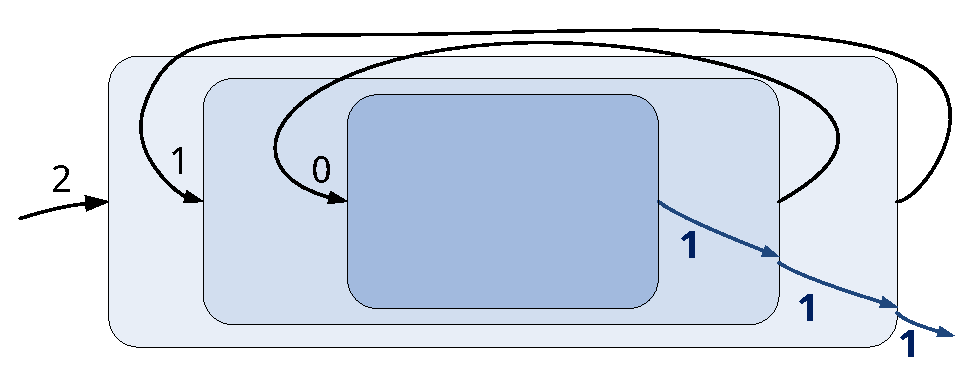
\includegraphics[height=1.0in]{figures/recursion.pdf}
\caption{Recursive Composition.\label{fig:recursion}}
\end{center}
\end{figure}

Here is the corresponding procedure:
\begin{schemedisplay}
(define g 
  (lambda (n)  
    (if (= n 0) 1 (g (- n 1)))))
\end{schemedisplay}

Unlike the earlier circular \scheme|f| procedure, if we apply \scheme|g| to any non-negative integer it will eventually produce an output.  For example, consider evaluating \scheme|(g 2)|.  When we evaluate the first application, the value of the parameter \scheme|n| is \schemeresult|2|, so the predicate expression \scheme|(= n 0)| evaluates to \schemeresult|false| and the value of the procedure body is the value of the alternate expression, \scheme|(g (- n 1))|.  The subexpression, \scheme|(- n 1)| evaluates to \schemeresult|1|, so the result is the result of applying \scheme|g| to \schemeresult|1|.  As with the previous application, this leads to the application, \scheme|(g (- n 1))|, but this time the value of \scheme|n| is \schemeresult|1|, so \scheme|(- n 1)| evaluates to \schemeresult|0|.  The next application leads to the application, \scheme|(g 0)|.  This time, the predicate expression evaluates to \schemeresult|true| and we have reached the base case.  The consequent expression is just \scheme|1|, so no further applications of \scheme|g| are performed and this is the result of the application \scheme|(g 0)|.  This is returned as the result of the \scheme|(g 1)| application in the previous recursive call, and then as the output of the original \scheme|(g 2)| application.

We can think of the recursive evaluation as winding until the base case is reached, and then unwinding the outputs back to the original application.  For this procedure, the output is not very interesting: no matter what positive number we apply \scheme|g| to, the eventual result is \schemeresult|1|.  To solve interesting problems with recursive procedures, we need to accumulate results as the recursive applications wind or unwind.  Examples~\ref{ex:factorial} and~\ref{ex:maximum} illustrate recursive procedures that accumulate the result during the unwinding process.  Example~\ref{ex:gcd} illustrates a recursive procedure that accumulates the result during the winding process.

\begin{example}{Factorial}\label{ex:factorial}\index{general}{factorial}
How many different arrangements are there of a deck of 52 playing cards?  

The top card in the deck can be any of the 52 cards, so there are 52 possible choices for the top card.  \sidepicturenocap{0.17}{images/shuffle-iStock_000000698868XSmall.jpg} 
The second card can be any of the cards except for the card that is the top card, so there are 51 possible choices for the second card.  The third card can be any of the 50 remaining cards, and so on, until the last card for which there is only one choice remaining.  
\begin{displaymath}
52 * 51 * 50 * \cdots * 2 * 1
\end{displaymath}
This is known as the \definition{factorial} function (denoted in mathematics using the exclamation point, e.g., $52!$).  It can be defined recursively:
\begin{quote}
$0! = 1$\\
$n! = n * (n - 1)!$ for all $n > 0$
\end{quote}
%n! = \left\{ \begin{array}{r@{\quad:\quad}l}
%1 & n=0 \\
%n * (n-1)! & n > 0
%\end{array} \right. 
%\]
The mathematical definition of factorial is recursive, so it is natural that we can define a recursive procedure that computes factorials:
\begin{schemedisplay}
(define (factorial n)
  (if (= n 0) 
     1
     (* n (factorial (- n 1)))))
\end{schemedisplay}

Evaluating \scheme|(factorial 52)| produces the number of arrangements of a 52-card deck: a sixty-eight digit number starting with an \scheme|8|.

The \scheme|factorial| procedure has structure very similar to our earlier definition of the useless recursive \scheme|g| procedure.  The only difference is the alternative expression for the if expression: in \scheme|g| we used \scheme|(g (- n 1))|; in \scheme|factorial| we added the outer application of \scheme|*|: 
\scheme|(* n (factorial (- n 1)))|.  Instead of just evaluating to the result of the recursive application, we are now combining the output of the recursive evaluation with the input \scheme|n| using a multiplication application.  
\end{example}

\beforeex
\begin{exercise}\label{ex:nchoosek}
How many different ways are there of choosing an unordered 5-card hand from a 52-card deck?  

This is an instance of the ``$n$ choose $k$'' problem (also known as the binomial coefficient): how many different ways are there to choose a set of $k$ items from $n$ items.  There are $n$ ways to choose the first item, $n - 1$ ways to choose the second, $\ldots$, and $n - k + 1$ ways to choose the $k^{th}$ item.  But, since the order does not matter, some of these ways are equivalent.  The number of possible ways to order the $k$ items is $k!$, so we can compute the number of ways to choose $k$ items from a set of $n$ items as:
\[
\frac{n * (n - 1) * \cdots * (n - k + 1)}{k!} = \frac{n!}{(n-k)!k!}
\]
\begin{subexerciselist}
\item \greenstar Define a procedure \scheme|choose| that takes two inputs, $n$ (the size of the item set) and $k$ (the number of items to choose), and outputs the number of possible ways to choose $k$ items from $n$.
\solution{
\begin{schemedisplay}
(define (choose n k)
   (/ (factorial n) (* (factorial (- n k)) (factorial k))))
\end{schemedisplay}
}
\item \bluestar Compute the number of possible 5-card hands that can be dealt from a 52-card deck.
\solution{
\begin{code}
\scheme|> (choose 52 5)|\\
\tb{\schemeresult|2598960|}\\
\end{code}
}
\item \goldstar Compute the likelihood of being dealt a flush (5 cards all of the same suit).  In a standard 52-card deck, there are 13 cards of each of the four suits.  Hint: divide the number of possible flush hands by the number of possible hands.
\solution{
The number of possible flushes for each suit is the number of ways to choose 5 cards from the 13 cards of each suit.  So the total number of possible flushes is \scheme|(* 4 (choose 13 5))|.  To compute the probability of being dealt a 5-card flush, we divide the number of ways to make a flush by the number of 5-card hands:
\begin{code}
\scheme|> (/ (* 4 (choose 13 5)) (choose 52 5))|\\
\tb{\schemeresult|33/16660|}\\
\scheme|> (exact->inexact (/ (* 4 (choose 13 5)) (choose 52 5)))|\\
\tb{\schemeresult|0.0019807923169267707|}\\
\end{code}
So, you should expect to see a 5-card flush roughly once every 505 hands.
}
\end{subexerciselist}
\end{exercise}
\afterex

\beforesplitex
\begin{exercise}\greenstar\label{ex:gauss-sum}\index{people}{Gauss, Karl}
Reputedly, when Karl Gauss was in elementary school his teacher assigned the class the task of summing the integers from 1 to 100 (e.g., $1 + 2 + 3 + \cdots + 100$) to keep them busy.  Being the (future) ``Prince of Mathematics'', Gauss developed the formula for calculating this sum, that is now known as the \emph{Gauss sum}.   
Had he been a computer scientist, however, and had access to a Scheme interpreter in the late 1700s, he might have instead defined a recursive procedure to solve the problem. Define a recursive procedure, \scheme|gauss-sum|, that takes a number \scheme|n| as its input parameter, and evaluates to the sum of the integers from 1 to \scheme|n| as its output.  For example, \scheme|(gauss-sum 100)| should evaluate to \schemeresult|5050|.
\solution{
\begin{schemedisplay}
(define (gauss-sum n)
   (if (= n 1) 1
       (+ n (gauss-sum (- n 1)))))
\end{schemedisplay}
}
\end{exercise}
\aftersplitex
\sidepicture{0.22}{images/gauss.jpg}{Karl Gauss}{} %http://en.wikipedia.org/wiki/File:Bendixen_-_Carl_Friedrich_Gau%C3%9F,_1828.jpg 

\beforesplitex
\begin{exercise}\goldstar\index{general}{accumulate}
Define a higher-order procedure, \scheme|accumulate|, that can be used to make both \scheme|gauss-sum| (from Exercise~\ref{ex:gauss-sum}) and \scheme|factorial|.  The \scheme|accumulate| procedure should take as its input the function used for accumulation (e.g., \scheme|*| for \scheme|factorial|, \scheme|+| for \scheme|gauss-sum|).  With your \scheme|accumulate| procedure, \scheme|((accumulate +) 100)| should evaluate to \schemeresult|5050| and \scheme|((accumulate *) 3)| should evaluate to \schemeresult|6|.  We assume the result of the base case is \scheme|1| (although a more general procedure could take that as a parameter).

Hint: since your procedure should produce a procedure as its output, it could start like this:
\begin{schemedisplay}
(define (accumulate f)
  (lambda (n) 
     (if (= n 1) 1
         ... 
\end{schemedisplay}
\solution{
\begin{schemedisplay}
(define (accumulate f)
   (lambda (n)
       (if (= n 1) 1
           (f n ((accumulate f) (- n 1))))))
\end{schemedisplay}
Here are a few examples:
\begin{code}
\scheme|> ((accumulate +) 100)|\\
\tb{\schemeresult|5050|}\\
\scheme|> ((accumulate +) 100)|\\
\tb{\schemeresult|5050|}\\
\scheme|> ((accumulate (lambda (x y) (- x y))) 10)|\\
\tb{\schemeresult|5|}\\
\end{code}           
}
\end{exercise}
\aftersplitex


\begin{examplenobar}{Find Maximum\label{ex:maximum}}
Consider the problem of defining a procedure that takes as its input a procedure, a low value, and a high value, and outputs the maximum value the input procedure produces when applied to an integer value between the low value and high value input.  We name the inputs \scheme|f|, \scheme|low|, and \scheme|high|. To find the maximum, the \scheme|find-maximum| procedure should evaluate the input procedure \scheme|f| at every integer value between the \scheme|low| and \scheme|high|, and output the greatest value found.  

Here are a few examples:
\begin{code}
\scheme|> (find-maximum (lambda (x) x) 1 20)|\\
\tb{\schemeresult|20|}\\
\scheme|> (find-maximum (lambda (x) (- 10 x)) 1 20)|\\
\tb{\schemeresult|9|}\\
\scheme|> (find-maximum (lambda (x) (* x (- 10 x))) 1 20)|\\
\tb{\schemeresult|25|}
\end{code}

To define the procedure, think about how to combine results from simpler problems to find the result.  For the base case, we need a case so simple we already know the answer.  Consider the case when \scheme|low| and \scheme|high| are equal.  Then, there is only one value to use, and we know the value of the maximum is \scheme|(f low)|.  So, the base case is \scheme|(if (= low high) (f low) ...)|.

How do we make progress towards the base case?  Suppose the value of \scheme|high| is equal to the value of \scheme|low| plus 1.  Then, the maximum value is either the value of \scheme|(f low)| or the value of \scheme|(f (+ low 1))|.  We could select it using the \scheme|bigger| procedure (from Example~\ref{example:bigger}): \scheme|(bigger (f low) (f (+ low 1)))|.  We can extend this to the case where \scheme|high| is equal to \scheme|low| plus 2:
\begin{schemedisplay}
(bigger (f low) (bigger (f (+ low 1)) (f (+ low 2))))
\end{schemedisplay}

The second operand for the outer \scheme|bigger| evaluation is the maximum value of the input procedure between the low value plus one and the high value input.  If we name the procedure we are defining \scheme|find-maximum|, then this second operand is the result of \scheme|(find-maximum f (+ low 1) high)|.  This works whether \scheme|high| is equal to \scheme|(+ low 1)|, or \scheme|(+ low 2)|, or any other value greater than \scheme|high|.  

Putting things together, we have our recursive definition of \scheme|find-maximum|:
\begin{schemedisplay}
(define (find-maximum f low high)
  (if (= low high) 
    (f low)
    (bigger (f low) (find-maximum f (+ low 1) high))))
\end{schemedisplay}
\end{examplenobar}

\beforesplitex
\begin{exercise}\greenstar
To find the maximum of a function that takes a real number as its input, we need to evaluate at all numbers in the range, not just the integers.  There are infinitely many numbers between any two numbers, however, so this is impossible.  We can approximate this, however, by evaluating the function at many numbers in the range.  

Define a procedure \scheme|find-maximum-epsilon| that takes as input a function \scheme|f|, a low range value \scheme|low|, a high range value \scheme|high|, and an increment \scheme|epsilon|, and produces as output the maximum value of \scheme|f| in the range between \scheme|low| and \scheme|high| at interval \scheme|epsilon|.  As the value of \scheme|epsilon| decreases, \scheme|find-maximum-epsilon| should evaluate to a value that approaches the actual maximum value. 

For example, 
\begin{schemedisplay}
(find-maximum-epsilon (lambda (x) (* x (- 5.5 x))) 1 10 1)
\end{schemedisplay}
evaluates to \schemeresult|7.5|.  And,
\begin{schemedisplay}
(find-maximum-epsilon (lambda (x) (* x (- 5.5 x))) 1 10 0.01)
\end{schemedisplay}
evaluates to \schemeresult|7.5625|.
\solution{
We start from the \scheme|find-maximum| definition from the example, and add an extra parameter:
\begin{schemedisplay}
(define (find-maximum-epsilon f low high epsilon)
  (if (>= low high) 
    (f low)
    (bigger (f low) (find-maximum-epsilon f (+ low epsilon) high epsilon))))
\end{schemedisplay}
The most important change is replacing \scheme|=| in the if expression predicate with \scheme|>=|.  Otherwise, it is possible the exact matching value is skipped and the procedure will continue to evaluate forever without every reaching the base case!
}
\end{exercise}
\aftersplitex

\beforeex
\begin{exercise}\goldstar
The \scheme|find-maximum| procedure we defined evaluates to the maximum value of the input function in the range, but does not provide the input value that produces that maximum output value.  Define a procedure that finds the input in the range that produces the maximum output value.  For example, \scheme|(find-maximum-input inc 1 10)| should evaluate to \scheme|10| and \scheme|(find-maximum-input (lambda (x) (* x (- 5.5 x))) 1 10)| should evaluate to \scheme|3|.
\solution{
%This one gets more complicated.  We need an extra parameter to keep track of the input that produces the maximum output value found so far.  To keep the interface the same, we define a worker procedure that takes the extra parameter, starting with the value of \scheme|low|.
%\begin{schemedisplay}
%(define (find-maximum-input f low high)
%  (define (find-maximum-input-worker f low high best)
%    (if (= low high) 
%        (if (> (f low) (f best)) 
%            low 
%            best)
%        (find-maximum-input-worker
%         f (+ low 1) high 
%         (if (> (f low) (f best)) low best))))
%  (find-maximum-input-worker f low high low))
%\end{schemedisplay}
(define (find-maximum-input f low high)
  (define (bigger-input a b)
    (if (> (f a) (f b)) a b))

  (if (= low high)
      low
      (bigger-input low (find-maximum-input f (+ low 1) high))))
}
% thanks to Ervin Varga for this solution which is much better than the original one!
\end{exercise}
\afterex

\beforeex
\begin{exercise}\goldstar
Define a \scheme|find-area| procedure that takes as input a function \scheme|f|, a low range value \scheme|low|, a high range value \scheme|high|, and an increment \scheme|epsilon|, and produces as output an estimate for the area under the curve produced by the function \scheme|f| between \scheme|low| and \scheme|high| using the \scheme|epsilon| value to determine how many regions to evaluate.
\solution{
We estimate the area under the curve by summing the areas of each trapezoid formed by the points $(x, 0)$, $(x, f(x))$, $(x + \epsilon, 0)$, $(x + \epsilon, f(x + \epsilon))$.  The area of a trapezoid is its length times its average height: $$\epsilon \times \frac{(f(x + \epsilon) - f(x))}{2}.$$  

\begin{schemedisplay}
(define (find-area f low high epsilon)
  (if (>= low high)
      0
      (+ (* (/ (+ (f low) (f (+ low epsilon))) 2) epsilon)
         (find-area f (+ low epsilon) high epsilon))))
\end{schemedisplay}
Here are some examples:
\begin{code}
\scheme|> (find-area (lambda (x) 5) 0 5 0.001)|\\
\tb{\schemeresult|24.99999999999931|}\\
\scheme|> (find-area (lambda (x) x) 0 5 0.001)|\\
\tb{\schemeresult|12.49999999999935|}\\
\scheme|> (find-area (lambda (x) (sin x)) 0 (* 2 pi) 0.0001)|\\
\tb{\schemeresult|1.0372978290178584e-010|}\\
\end{code}
The answers are not exact for two reasons.  The first is that epsilon is not infinitesimal (and never can be with a finite computation).  The second is a minor bug in the code since it does not account for the situation where \scheme|(+ low epsilon)| exceeds \scheme|high|.  Fixing this problem is left as (another) exercise for the reader.
}
\end{exercise}
\afterex

\begin{examplenobar}{Euclid's Algorithm\label{ex:gcd}}\index{people}{Euclid} In Book 7 of the \emph{Elements}, Euclid describes an algorithm for finding the greatest common divisor of two non-zero integers.  The greatest common divisor is the greatest integer that divides both of the input numbers without leaving any remainder.  For example, the greatest common divisor of 150 and 200 is 50 since \scheme|(/ 150 50)| evaluates to \schemeresult|3| and \scheme|(/ 200 50)| evaluates to \schemeresult|4|, and there is no number greater than 50 that can evenly divide both 150 and 200.  

\index{general}{modulo} The \scheme|modulo| primitive procedure takes two integers as its inputs and evaluates to the remainder when the first input is divided by the second input.  For example, \scheme|(modulo 6 3)| evaluates to \schemeresult|0| and \scheme|(modulo 7 3)| evaluates to \schemeresult|1|.

Euclid's algorithm stems from two properties of integers:
\begin{enumtight}
\item If \scheme|(modulo a b)| evaluates to 0 then \scheme|b| is the greatest common divisor of \scheme|a| and \scheme|b|.  
\item If \scheme|(modulo a b)| evaluates to a non-zero integer \emph{r}, the greatest common divisor of \scheme|a| and \scheme|b| is the greatest common divisor of \scheme|b| and \emph{r}.
\end{enumtight}
We can define a recursive procedure for finding the greatest common divisor closely following Euclid's algorithm\footnote{DrRacket provides a built-in procedure \scheme|gcd| that computes the greatest common divisor.  We name our procedure \scheme|gcd-euclid| to avoid a clash with the build-in procedure.}:
\begin{schemedisplay}
(define (gcd-euclid a b) 
  (if (= (modulo a b) 0) b (gcd-euclid b (modulo a b))))
\end{schemedisplay}
The structure of the definition is similar to the \scheme|factorial| definition: the procedure body is an if expression and the predicate tests for the base case.  For the \scheme|gcd-euclid| procedure, the base case corresponds to the first property above.  It occurs when \scheme|b| divides \scheme|a| evenly, and the consequent expression is \scheme|b|.  The alternate expression, \scheme|(gcd-euclid b (modulo a b))|, is the recursive application.  

The \scheme|gcd-euclid| procedure differs from the \scheme|factorial| definition in that there is no outer application expression in the recursive call.  We do not need to combine the result of the recursive application with some other value as was done in the \scheme|factorial| definition, the result of the recursive application is the final result.  Unlike the \scheme|factorial| and \scheme|find-maximum| examples, the \scheme|gcd-euclid| procedure produces the result in the base case, and no further computation is necessary to produce the final result.  When no further evaluation is necessary to get from the result of the recursive application to the final result, a recursive definition is said to be \definition{tail recursive}.  Tail recursive procedures have the advantage that they can be evaluated without needing to keep track of the stack of previous recursive calls.  Since the final call produces the final result, there is no need for the interpreter to unwind the recursive calls to produce the answer. 

\beforeex
\begin{exercise}
Show the structure of the \scheme|gcd-euclid| applications in evaluating \scheme|(gcd-euclid 6 9)|.
\solution{
The first application is \scheme|(gcd-euclid 6 9)|.  Since the predicate is false, the alternate clause is evaluated.  It leads to the application \scheme|(gcd-euclid 9 6)|.  In this application, the predicate is still false, and the alernate clause is valuated.  Since \scheme|(modulo 9 6)| evaluates to \scheme|3|, this results in the application \scheme|(gcd-euclid 6 3)|.  For this application, the predicate is \scheme|(= (modulo 6 3) 0)| which is \scheme|true|.  Hence, the expression evaluates to the consequence clause, \scheme|b| which has the value \schemeresult|3|.
}
\end{exercise}
\afterex

\beforeex
\begin{exercise}\goldstar
Provide a convincing argument why the evaluation of \scheme|(gcd-euclid a b)| will always finish when the inputs are both positive integers.
\solution{
\LATER{}
}
\end{exercise}
\afterex

\beforeex
\begin{exercise}\greenstar
Provide an alternate definition of \scheme|factorial| that is tail recursive.  To be tail recursive, the expression containing the recursive application cannot be part of another application expression.  
(Hint: define a \scheme|factorial-helper| procedure that takes an extra parameter, and then define \scheme|factorial| as \scheme|(define (factorial n) (factorial-helper n 1))|.)
\solution{
Following the hint, we add an extra parameter to keep track of the working result:
\begin{schemedisplay}
(define (factorial n)
   (define (factorial-helper n v)
      (if (= n 1) v
          (factorial-helper (- n 1) (* v n))))
   (factorial-helper n 1))
\end{schemedisplay}
}
\end{exercise}
\afterex

\beforeex
\begin{exercise}\greenstar
Provide a tail recursive definition of \scheme|find-maximum|.
\solution{
\begin{schemedisplay}
(define (find-maximum-tail f low high)
  (define (find-maximum-helper f low high best)    
    (if (= low high) 
        (bigger (f low) best)
        (find-maximum-helper f (+ low 1) high (bigger (f low) best))))
  (find-maximum-helper f low high (f low)))
\end{schemedisplay}
}
\end{exercise}
\afterex

\beforeex
\begin{exercise}\doublegoldstar
Provide a convincing argument why it is possible to transform any recursive procedure into an equivalent procedure that is tail recursive.
\solution{
\LATER{}
}
\end{exercise}
\afterex

\end{examplenobar}

%%! \clearpage %%!
\splitexplore{Square Roots}{\label{exploration:sqrt}\index{general}{square root}\index{people}{Newton, Isaac}\index{people}{Heron}  One of the earliest known algorithms is a method for computing square roots.  It is known as Heron's method after the Greek mathematician Heron of Alexandria who lived in the first century AD who described the method, although it was also known to the Babylonians many centuries earlier.  Isaac Newton developed a more general method for estimating functions based on their derivatives known as Netwon's method, of which Heron's method is a specialization.  

Square root is a mathematical function that take a number, $a$, as input and outputs a value $x$ such that $x^2 = a$.  For many numbers (including 2), the square root is irrational, so the best we can hope for with is a good approximation.  We define a procedure \scheme|find-sqrt| that takes the target number as input and outputs an approximation for its square root.

Heron's method works by starting with an arbitrary guess, $g_0$.  Then, with each iteration, compute a new guess ($g_n$ is the $n^{th}$ guess) that is a function of the previous guess ($g_{n - 1}$) and the target number ($a$):
\begin{displaymath}
g_n = \frac{g_{n - 1} + \frac{a}{g_{n - 1}}}{2}
\end{displaymath}
As $n$ increases $g_n$ gets closer and closer to the square root of $a$.

The definition is recursive since we compute $g_n$ as a function of $g_{n-1}$, so we can define a recursive procedure that computes Heron's method.  First, we define a procedure for computing the next guess from the previous guess and the target:
\sidepicture{0.3}{images/Heron.jpg}{Heron of Alexandria}{} % http://en.wikipedia.org/wiki/File:Heron.jpeg
\begin{schemedisplay}
(define (heron-next-guess a g) (/ (+ g (/ a g)) 2))
\end{schemedisplay}
Next, we define a recursive procedure to compute the $n^{th}$ guess using Heron's method.  It takes three inputs: the target number, $a$, the number of guesses to make, $n$, and the value of the first guess, $g$.
\begin{schemedisplay}
(define (heron-method a n g)
  (if (= n 0)
      g
      (heron-method a (- n 1) (heron-next-guess a g))))
\end{schemedisplay}
To start, we need a value for the first guess.  The choice doesn't really matter --- the method works with any starting guess (but will reach a closer estimate quicker if the starting guess is good).  We will use \scheme|1| as our starting guess.  So, we can define a \scheme|find-sqrt| procedure that takes two inputs, the target number and the number of guesses to make, and outputs an approximation of the square root of the target number.
\begin{schemedisplay}
(define (find-sqrt a guesses)
  (heron-method a guesses 1))
\end{schemedisplay}
Heron's method converges to a good estimate very quickly:
\begin{code}
\scheme|> (square (find-sqrt 2 0))|\\
\schemeresult|1|\\
\scheme|> (square (find-sqrt 2 1))|\\
\schemeresult|2 1/4|\\
\scheme|> (square (find-sqrt 2 2))|\\
\schemeresult|2 1/144|\\
\scheme|> (square (find-sqrt 2 4))|\\
\schemeresult|2 1/221682772224|\\
\scheme|> (exact->inexact (find-sqrt 2 5))|\\
\schemeresult|1.4142135623730951|\\
\end{code}
The actual square root of 2 is $1.414213562373095048\ldots$, so our estimate is correct to 16 digits after only five guesses.

Users of square roots don't really care about the method used to find the square root (or how many guesses are used).  Instead, what is important to a square root user is how close the estimate is to the actual value.  Can we change our \scheme|find-sqrt| procedure so that instead of taking the number of guesses to make as its second input it takes a minimum tolerance value?

Since we don't know the actual square root value (otherwise, of course, we could just return that), we need to measure tolerance as how close the square of the approximation is to the target number.  Hence, we can stop when the square of the guess is close enough to the target value.
\begin{schemedisplay}
(define (close-enough? a tolerance g)
  (<= (abs (- a (square g))) tolerance))
\end{schemedisplay}
The stopping condition for the recursive definition is now when the guess is close enough.  Otherwise, our definitions are the same as before.
\begin{schemedisplay}
(define (heron-method-tolerance a tolerance g)
  (if (close-enough? a tolerance g) 
      g
      (heron-method-tolerance a tolerance (heron-next-guess a g))))

(define (find-sqrt-approx a tolerance)
  (heron-method-tolerance a tolerance 1))
\end{schemedisplay}
Note that the value passed in as \scheme|tolerance| does not change with each recursive call.  We are making the problem smaller by making each successive guess closer to the required answer.

Here are some example interactions with \scheme|find-sqrt-approx|:
\begin{code}
\scheme|> (exact->inexact (square (find-sqrt-approx 2 0.01)))|\\
\schemeresult|2.0069444444444446|\\
\scheme|> (exact->inexact (square (find-sqrt-approx 2 0.0000001)))|\\
\schemeresult|2.000000000004511|
\end{code}

%\excur{How much does the initial guess (we used the value \scheme|1|) in Heron's method matter?  Try answering this both experimentally and analytically.  Can you improve the \scheme|find-sqrt| procedure by using a better initial guess?}

\begin{subexerciselist}
\item How accurate is the built-in \scheme|sqrt| procedure?
\item Can you produce more accurate square roots than the built-in \scheme|sqrt| procedure? 
\item Why doesn't the built-in procedure do better?
\end{subexerciselist}
}

\section{Evaluating Recursive Applications}

Evaluating an application of a recursive procedure follows the evaluation rules just like any other expression evaluation.  It may be confusing, however, to see that this works because of the apparent circularity of the procedure definition.  

Here, we show in detail the evaluation steps for evaluating \scheme|(factorial 2)|.  The evaluation and application rules refer to the rules summary in Section~\ref{sec:rules}.  We first show the complete evaluation following the substitution model evaluation rules in full gory detail, and later review a subset showing the most revealing steps.  Stepping through even a fairly simple evaluation using the evaluation rules is quite tedious, and not something humans should do very often (that's why we have computers!) but instructive to do once to understand exactly how an expression is evaluated.

The evaluation rule for an application expression does not specify the order in which the subexpressions are evaluated.  A Scheme interpreter is free to evaluate them in any order.  Here, we choose to evaluate the subexpressions in the order that is most readable.  The value produced by an evaluation does not depend on the order in which the subexpressions are evaluated.\footnote{This is only true for the subset of Scheme we have defined so far.  Once we introduce side effects and mutation, it is no longer the case, and expressions can produce different results depending on the order in which they are evaluated.}

In the evaluation steps, we use \texttt{typewriter} font for uninterpreted Scheme expressions and \sresult{sans-serif} font to show values. So, \texttt{2} represents the Scheme expression that evaluates to the number \sresult{2}.

\vspace*{\baselineskip}
%%!\newpage 

\evalstart
\evalstepa {{\underline{(factorial 2)}}}{Evaluation Rule 3(a): Application subexpressions}
\evalstepa {(\underline{factorial} 2)}{Evaluation Rule 2: Name}
\evalstepb {(\underline{(lambda (n) (if (= n 0) 1 (* n (factorial (- n 1)))))} 2)}{Evaluation Rule 4: Lambda}
\evalstepa {(\sresult{(lambda (n) (if (= n 0) 1 (* n (factorial (- n 1)))))} \underline{2})}{Evaluation Rule 1: Primitive}
\evalstepb {\underline{(\sresult{(lambda (n) (if (= n 0) 1 (* n (factorial (- n 1)))))} \sresult{2})}}{Evaluation Rule 3(b): Application, Application Rule 2} 
\evalstepa {(if \underline{(= \sresult{2} 0)} 1 (* \sresult{2} (factorial (- \sresult{2} 1))))}{Evaluation Rule 5(a): If predicate} 
\evalstepb {(if \underline{(= \sresult{2} 0)} 1 (* \sresult{2} (factorial (- \sresult{2} 1))))}{Evaluation Rule 3(a): Application subexpressions}
\evalstepa {(if (\underline{=} \sresult{2} \underline{0}) 1 (* \sresult{2} (factorial (- \sresult{2} 1))))}{Evaluation Rule 1: Primitive}
\evalstepb {(if \underline{(\sresult{=} \sresult{2} \sresult{0})} 1 (* \sresult{2} (factorial (- \sresult{2} 1))))}{Evaluation Rule 3(b): Application, Application Rule 1}
\evalstepa {\underline{(if \sresult{false} 1 (* \sresult{2} (factorial (- \sresult{2} 1))))}}{Evaluation Rule 5(b): If alternate}
\evalstepa {\underline{(* \sresult{2} (factorial (- \sresult{2} 1)))}}{Evaluation Rule 3(a): Application subexpressions}
\evalstepa {(\underline{*} \sresult{2} (factorial (- \sresult{2} 1)))}{Evaluation Rule 1: Primitive}
\evalstepa {(\sresult{*} \sresult{2} \underline{(factorial (- \sresult{2} 1))})}{Evaluation Rule 3(a): Application subexpressions}
\evalstepa {(\sresult{*} \sresult{2} (factorial \underline{(- \sresult{2} 1)}))}{Evaluation Rule 3(a): Application subexpressions}
\evalstepa {(\sresult{*} \sresult{2} (factorial (\underline{-} \sresult{2} \underline{1})))}{Evaluation Rule 1: Primitive}
\evalstepa {(\sresult{*} \sresult{2} (factorial (\sresult{-} \sresult{2} \sresult{1})))}{Evaluation Rule 3(b): Application, Application Rule 1}
\evalindent
\evalstepa {(\sresult{*} \sresult{2} (\underline{factorial} \sresult{1}))}{Continue Evaluation Rule 3(a); Evaluation Rule 2: Name}
\evalstepb {(\sresult{*} \sresult{2} (\underline{(lambda (n) (if (= n 0) 1 (* n (factorial (- n 1)))))} \sresult{1}))}{Evaluation Rule 4: Lambda} %%tiny
\evalstepb {(\sresult{*} \sresult{2} \underline{(\sresult{(lambda (n) (if (= n 0) 1 (* n (factorial (- n 1)))))} \sresult{1})})} {Evaluation Rule 3(b): Application, Application Rule 2}
\evalstepb {(\sresult{*} \sresult{2} \underline{(if (= \sresult{1} 0) 1 (* \sresult{1} (factorial (- \sresult{1} 1))))})} {Evaluation Rule 5(a): If predicate}
\evalstepb {(\sresult{*} \sresult{2} (if \underline{(= \sresult{1} 0)} 1 (* \sresult{1} (factorial (- \sresult{1} 1)))))} {Evaluation Rule 3(a): Application subexpressions}
\evalstepb {(\sresult{*} \sresult{2} (if (\underline{=} \sresult{1} \underline{0}) 1 (* \sresult{1} (factorial (- \sresult{1} 1)))))} {Evaluation Rule 1: Primitives}
\evalstepb {(\sresult{*} \sresult{2} (if \underline{(\sresult{=} \sresult{1} \sresult{0})} 1 (* \sresult{1} (factorial (- \sresult{1} 1)))))} {Evaluation Rule 3(b): Application Rule 1}
\evalstepb {(\sresult{*} \sresult{2} \underline{(if \sresult{false} 1 (* \sresult{1} (factorial (- \sresult{1} 1))))})} {Evaluation Rule 5(b): If alternate}
\evalstepa {(\sresult{*} \sresult{2} \underline{(* \sresult{1} (factorial (- \sresult{1} 1)))})} {Evaluation Rule 3(a): Application}
\evalstepa {(\sresult{*} \sresult{2} (\underline{*} \underline{1} (factorial (- \sresult{1} 1))))} {Evaluation Rule 1: Primitives}
\evalstepa {(\sresult{*} \sresult{2} (\sresult{*} \sresult{1} \underline{(factorial (- \sresult{1} 1))}))} {Evaluation Rule 3(a): Application}
\evalstepa {(\sresult{*} \sresult{2} (\sresult{*} \sresult{1} (factorial \underline{(- \sresult{1} 1)})))} {Evaluation Rule 3(a): Application}
\evalstepa {(\sresult{*} \sresult{2} (\sresult{*} \sresult{1} (factorial (\underline{-} \sresult{1} \underline{1}))))} {Evaluation Rule 1: Primitives}
\evalstepb {(\sresult{*} \sresult{2} (\sresult{*} \sresult{1} (factorial \underline{(\sresult{-} \sresult{1} \sresult{1})})))} {Evaluation Rule 3(b): Application, Application Rule 1}
\evalindent
\evalstepa {(\sresult{*} \sresult{2} (\sresult{*} \sresult{1} (\underline{factorial} \sresult{0})))} {Evaluation Rule 2: Name}
\evalstepb {(\sresult{*} \sresult{2} (\sresult{*} \sresult{1} (\underline{(lambda (n) (if (= n 0) 1 (* n (fact... ))))} \sresult{0})))} {Evaluation Rule 4, Lambda}
\evalstepb {(\sresult{*} \sresult{2} (\sresult{*} \sresult{1} \underline{(\sresult{(lambda (n) (if (= n 0) 1 (* n (factorial (- n 1)))))} \sresult{0})}))} {Evaluation Rule 3(b), Application Rule 2}
\evalstepb {(\sresult{*} \sresult{2} (\sresult{*} \sresult{1} \underline{(if (= \sresult{0} 0) 1 (* \sresult{0} (factorial (- \sresult{0} 1))))}))} {Evaluation Rule 5(a): If predicate}
\evalstepb {(\sresult{*} \sresult{2} (\sresult{*} \sresult{1} (if \underline{(= \sresult{0} 0)} 1 (* \sresult{0} (factorial (- \sresult{0} 1))))))} {Evaluation Rule 3(a): Application subexpressions}
\evalstepb {(\sresult{*} \sresult{2} (\sresult{*} \sresult{1} (if (\underline{=} \sresult{0} \underline{0}) 1 (* \sresult{0} (factorial (- \sresult{0} 1))))))} {Evaluation Rule 1: Primitives}
\evalstepb {(\sresult{*} \sresult{2} (\sresult{*} \sresult{1} (if \underline{(\sresult{=} \sresult{0} \sresult{0})} 1 (* \sresult{0} (factorial (- \sresult{0} 1))))))} {Evaluation Rule 3(b): Application, Application Rule 1}
\evalstepb {(\sresult{*} \sresult{2} (\sresult{*} \sresult{1} \underline{(if \sresult{true} 1 (* \sresult{0} (factorial (- \sresult{0} 1))))}))} {Evaluation Rule 5(b): If consequent}
\evalstepa {(\sresult{*} \sresult{2} (\sresult{*} \sresult{1} \underline{1}))} {Evaluation Rule 1: Primitives}
\evalstepa {(\sresult{*} \sresult{2} \underline{(\sresult{*} \sresult{1} \sresult{1})})} {Evaluation Rule 3(b): Application, Application Rule 1} 
\evalunindent
\evalstepa {\underline{(\sresult{*} \sresult{2} \sresult{1})}} {Evaluation Rule 3(b): Application, Application Rule 1}
\evalunindent
\evalstepa {\sresult{2}}{Evaluation finished, no unevaluated expressions remain.}
\evalend

The key to evaluating recursive procedure applications is if special evaluation rule.  If the if expression were evaluated like a regular application all subexpressions would be evaluated, and the alternative expression containing the recursive call would never finish evaluating!  Since the evaluation rule for if evaluates the predicate expression first and does not evaluate the alternative expression when the predicate expression is true, the circularity in the definition ends when the predicate expression evaluates to true.  This is the base case.  In the example, this is the base case where \scheme{(= n 0)} evaluates to true and instead of producing another recursive call it evaluates to \schemeresult|1|.

\shortsection{The Evaluation Stack} The structure of the evaluation is clearer from just the most revealing steps:

\evalstart
\revalstep {(factorial 2)}{Evaluation Rule 3(a): Application subexpressions}
	\hevalstep {(\underline{factorial} 2)}{Evaluation Rule 2: Name}
	\hevalsteptiny {(\underline{(lambda (n) (if (= n 0) 1 (* n (factorial (- n 1)))))} 2)}{Evaluation Rule 4: Lambda}
	\hevalstep {(\sresult{(lambda (n) (if (= n 0) 1 (* n (factorial (- n 1)))))} \underline{2})}{Evaluation Rule 1: Primitive}
	\hevalstep {\underline{(\sresult{(lambda (n) (if (= n 0) 1 (* n (factorial (- n 1)))))} \sresult{2})}}{Evaluation Rule 3(b): Application, Application Rule 2} 
	\hevalstep {(if \underline{(= \sresult{2} 0)} 1 (* \sresult{2} (factorial (- \sresult{2} 1))))}{Evaluation Rule 5(a): If predicate} 
	\hevalstep {(if \underline{(= \sresult{2} 0)} 1 (* \sresult{2} (factorial (- \sresult{2} 1))))}{Evaluation Rule 3(a): Application subexpressions}
	\hevalstep {(if (\underline{=} \sresult{2} \underline{0}) 1 (* \sresult{2} (factorial (- \sresult{2} 1))))}{Evaluation Rule 1: Primitive}
	\hevalstep {(if \underline{(\sresult{=} \sresult{2} \sresult{0})} 1 (* \sresult{2} (factorial (- \sresult{2} 1))))}{Evaluation Rule 3(b): Application, Application Rule 1}
	\hevalstep {\underline{(if \sresult{false} 1 (* \sresult{2} (factorial (- \sresult{2} 1))))}}{Evaluation Rule 5(b): If alternate}
	\hevalstep {\underline{(* \sresult{2} (factorial (- \sresult{2} 1)))}}{Evaluation Rule 3(a): Application subexpressions}
	\hevalstep {(\underline{*} \sresult{2} (factorial (- \sresult{2} 1)))}{Evaluation Rule 1: Primitive}
	\hevalstep {(\sresult{*} \sresult{2} \underline{(factorial (- \sresult{2} 1))})}{Evaluation Rule 3(a): Application subexpressions}
	\hevalstep {(\sresult{*} \sresult{2} (factorial \underline{(- \sresult{2} 1)}))}{Evaluation Rule 3(a): Application subexpressions}
	\hevalstep {(\sresult{*} \sresult{2} (factorial (\underline{-} \sresult{2} \underline{1})))}{Evaluation Rule 1: Primitive}
	\hevalstep {(\sresult{*} \sresult{2} (factorial (\sresult{-} \sresult{2} \sresult{1})))}{Evaluation Rule 3(b): Application, Application Rule 1}
\revalstep {\qquad(\sresult{*} \sresult{2} (factorial \sresult{1}))}{Continuing Evaluation Rule 3(a); Evaluation Rule 2: Name}
	\hevalsteptiny {(\sresult{*} \sresult{2} (\underline{(lambda (n) (if (= n 0) 1 (* n (factorial (- n 1)))))} \sresult{1}))}{Evaluation Rule 4: Lambda}
	\hevalstep {(\sresult{*} \sresult{2} \underline{(\sresult{(lambda (n) (if (= n 0) 1 (* n (factorial (- n 1)))))} \sresult{1})})} {Evaluation Rule 3(b): Application, Application Rule 2}
	\hevalstep {(\sresult{*} \sresult{2} \underline{(if (= \sresult{1} 0) 1 (* \sresult{1} (factorial (- \sresult{1} 1))))})} {Evaluation Rule 5(a): If predicate}
	\hevalstep {(\sresult{*} \sresult{2} (if \underline{(= \sresult{1} 0)} 1 (* \sresult{1} (factorial (- \sresult{1} 1)))))} {Evaluation Rule 3(a): Application subexpressions}
	\hevalstep {(\sresult{*} \sresult{2} (if (\underline{=} \sresult{1} \underline{0}) 1 (* \sresult{1} (factorial (- \sresult{1} 1)))))} {Evaluation Rule 1: Primitives}
	\hevalstep {(\sresult{*} \sresult{2} (if \underline{(\sresult{=} \sresult{1} \sresult{0})} 1 (* \sresult{1} (factorial (- \sresult{1} 1)))))} {Evaluation Rule 3(b): Application Rule 1}
	\hevalstep {(\sresult{*} \sresult{2} \underline{(if \sresult{false} 1 (* \sresult{1} (factorial (- \sresult{1} 1))))})} {Evaluation Rule 5(b): If alternate}
	\hevalstep {(\sresult{*} \sresult{2} \underline{(* \sresult{1} (factorial (- \sresult{1} 1)))})} {Evaluation Rule 3(a): Application}
	\hevalstep {(\sresult{*} \sresult{2} (\underline{*} \underline{1} (factorial (- \sresult{1} 1))))} {Evaluation Rule 1: Primitives}
	\hevalstep {(\sresult{*} \sresult{2} (\sresult{*} \sresult{1} \underline{(factorial (- \sresult{1} 1))}))} {Evaluation Rule 3(a): Application}
	\hevalstep {(\sresult{*} \sresult{2} (\sresult{*} \sresult{1} (factorial \underline{(- \sresult{1} 1)})))} {Evaluation Rule 3(a): Application}
	\hevalstep {(\sresult{*} \sresult{2} (\sresult{*} \sresult{1} (factorial (\underline{-} \sresult{1} \underline{1}))))} {Evaluation Rule 1: Primitives}
	\hevalstep {(\sresult{*} \sresult{2} (\sresult{*} \sresult{1} (factorial \underline{(\sresult{-} \sresult{1} \sresult{1})})))} {Evaluation Rule 3(b): Application, Application Rule 1}

\revalstep {\qquad\qquad(\sresult{*} \sresult{2} (\sresult{*} \sresult{1} (factorial \sresult{0})))} {Evaluation Rule 2: Name}
	\hevalsteptiny {(\sresult{*} \sresult{2} (\sresult{*} \sresult{1} (\underline{(lambda (n) (if (= n 0) 1 (* n (factorial (- n 1)))))} \sresult{0})))} {Evaluation Rule 4, Lambda}
	\hevalstep {(\sresult{*} \sresult{2} (\sresult{*} \sresult{1} \underline{(\sresult{(lambda (n) (if (= n 0) 1 (* n (factorial (- n 1)))))} \sresult{0})}))} {Evaluation Rule 3(b), Application Rule 2}
	\hevalstep {(\sresult{*} \sresult{2} (\sresult{*} \sresult{1} \underline{(if (= \sresult{0} 0) 1 (* \sresult{0} (factorial (- \sresult{0} 1))))}))} {Evaluation Rule 5(a): If predicate}
	\hevalstep {(\sresult{*} \sresult{2} (\sresult{*} \sresult{1} (if \underline{(= \sresult{0} 0)} 1 (* \sresult{0} (factorial (- \sresult{0} 1))))))} {Evaluation Rule 3(a): Application subexpressions}
	\hevalstep {(\sresult{*} \sresult{2} (\sresult{*} \sresult{1} (if (\underline{=} \sresult{0} \underline{0}) 1 (* \sresult{0} (factorial (- \sresult{0} 1))))))} {Evaluation Rule 1: Primitives}
	\hevalstep {(\sresult{*} \sresult{2} (\sresult{*} \sresult{1} (if \underline{(\sresult{=} \sresult{0} \sresult{0})} 1 (* \sresult{0} (factorial (- \sresult{0} 1))))))} {Evaluation Rule 3(b): Application, Application Rule 1}
	\hevalstep {(\sresult{*} \sresult{2} (\sresult{*} \sresult{1} \underline{(if \sresult{true} 1 (* \sresult{0} (factorial (- \sresult{0} 1))))}))} {Evaluation Rule 5(b): If consequent}
   \hevalstep {(\sresult{*} \sresult{2} (\sresult{*} \sresult{1} \underline{1}))} {Evaluation Rule 1: Primitives}
\revalstep {\qquad\qquad(\sresult{*} \sresult{2} (\sresult{*} \sresult{1} \sresult{1}))} {Evaluation Rule 3(b): Application, Application Rule 1}
\revalstep {\qquad(\sresult{*} \sresult{2} \sresult{1})} {Evaluation Rule 3(b): Application, Application Rule 1}
\revalstep {\sresult{2}}{Value reached}
\evalend

\index{general}{evaluation stack}
Step 1 starts evaluating \scheme|(factorial 2)|.  The result is found in Step 42.  To evaluate \scheme|(factorial 2)|, we follow the evaluation rules, eventually reaching the body expression of the if expression in the factorial definition in Step 17.  Evaluating this expression requires evaluating the \scheme|(factorial 1)| subexpression.  At Step 17, the first evaluation is in progress, but to complete it we need the value resulting from the second recursive application.  

Evaluating the second application results in the body expression, \scheme|(* 1 (factorial 0))|, shown for Step 31.  At this point, the evaluation of \scheme|(factorial 2)| is stuck in Evaluation Rule 3, waiting for the value of \scheme|(factorial 1)| subexpression.  The evaluation of the \scheme|(factorial 1)| application leads to the \scheme|(factorial 0)| subexpression, which must be evaluated before the \scheme|(factorial 1)| evaluation can complete.  

In Step 40, the \scheme|(factorial 0)| subexpression evaluation has completed and produced the value \schemeresult|1|.  Now, the \scheme|(factorial 1)| evaluation can complete, producing \schemeresult|1| as shown in Step 41.  Once the \scheme|(factorial 1)| evaluation completes, all the subexpressions needed to evaluate the expression in Step 17 are now evaluated, and the evaluation completes in Step 42.

Each recursive application can be tracked using a stack, similarly to processing RTN subnetworks (Section~\ref{sec:subnetworks}).  A stack has the property that the first item pushed on the stack will be the last item removed---all the items pushed on top of this one must be removed before this item can be removed.  For application evaluations, the elements on the stack are expressions to evaluate.  To finish evaluating the first expression, all of its component subexpressions must be evaluated.  Hence, the first application evaluation started is the last one to finish.\index{general}{recursive definition|)}

\beforesplitex
\begin{exercise}\label{ex:eval}
This exercise tests your understanding of the \scheme|(factorial 2)| evaluation. 
\begin{subexerciselist}
\item In step 5, the second part of the application evaluation rule, Rule 3(b), is used.  In which step does this evaluation rule complete?
\item In step 11, the first part of the application evaluation rule, Rule 3(a), is used.  In which step is the following use of Rule 3(b) started?
\item In step 25, the first part of the application evaluation rule, Rule 3(a), is used.  In which step is the following use of Rule 3(b) started?
\item \greenstar To evaluate \scheme|(factorial 3)|, how many times would Evaluation Rule 2 be used to evaluate the name \scheme|factorial|?
\item \goldstar To evaluate \scheme|(factorial n)| for any positive integer \scheme|n|, how many times would Evaluation Rule 2 be used to evaluate the name \scheme|factorial|?
\end{subexerciselist}
\end{exercise}
\aftersplitex

\beforesplitex
\begin{exercise}
For which input values \emph{n} will an evaluation of \scheme|(factorial n)| eventually reach a value?  For values where the evaluation is guaranteed to finish, make a convincing argument why it must finish.  For values where the evaluation would not finish, explain why.
\end{exercise}
\aftersplitex

\section{Developing Complex Programs}
To develop and use more complex procedures it will be useful to learn some helpful techniques for understanding what is going on when procedures are evaluated.  It is very rare for a first version of a program to be completely correct, even for an expert programmer.  Wise programmers build programs incrementally, by writing and testing small components one at a time.

The process of fixing broken programs is known as \definition{debugging}.  The key to debugging effectively is to be systematic and thoughtful.  It is a good idea to take notes to keep track of what you have learned and what you have tried.  Thoughtless debugging can be very frustrating, and is unlikely to lead to a correct program.  

A good strategy for debugging is to:
\begin{enumtight}
\item Ensure you understand the intended behavior of your procedure.  Think of a few representative inputs, and what the expected output should be.
\item Do experiments to observe the actual behavior of your procedure.  Try your program on simple inputs first.  What is the relationship between the actual outputs and the desired outputs?  Does it work correctly for some inputs but not others?  
\item Make changes to your procedure and retest it.  If you are not sure what to do, make changes in small steps and carefully observe the impact of each change.  
\end{enumtight}
\sidepicture{0.3}{images/hoppermoth.png}{First actual bug}{Grace Hopper's notebook, 1947}%http://en.wikipedia.org/wiki/File:H96566k.jpg
\index{people}{Hopper, Grace}

For more complex programs, follow this strategy at the level of sub-com\-po\-nents.  For example, you can try debugging at the level of one expression before trying the whole procedure.  Break your program into several procedures so you can test and debug each procedure independently.  The smaller the unit you test at one time, the easier it is to understand and fix problems. 

DrRacket provides many useful and powerful features to aid debugging, but the most important tool for debugging is using your brain to think carefully about what your program should be doing and how its observed behavior differs from the desired behavior.  Next, we describe two simple ways to observe program behavior.

\subsection{Printing}\label{sec:printing}\index{general}{printing}

One useful procedure built-in to DrRacket is the \scheme|display| procedure\index{general}{display}.  It takes one input, and produces no output.  Instead of producing an output, it prints out the value of the input (it will appear in purple in the Interactions window).  We can use \scheme|display| to observe what a procedure is doing as it is evaluated.  

For example, if we add a \scheme|(display n)| expression at the beginning of our \scheme|factorial| procedure we can see all the intermediate calls.  To make each printed value appear on a separate line, we use the \scheme|newline| procedure\index{general}{newline}.  The \scheme|newline| procedure prints a new line; it takes no inputs and produces no output.  

\begin{schemedisplay}
(define (factorial n)
  (display "Enter factorial: ") (display n) (newline)
  (if (= n 0) 1 (* n (factorial (- n 1)))))
\end{schemedisplay}

Evaluating \scheme|(factorial 2)| produces:
\begin{code}
\textcolor{purple}{\emph{Enter factorial: 2}}\\
\textcolor{purple}{\emph{Enter factorial: 1}}\\
\textcolor{purple}{\emph{Enter factorial: 0}}\\
\schemeresult{2}
\end{code}
\index{general}{printing}\index{general}{printf}
The built-in \scheme|printf| procedure makes it easier to print out many values at once.  It takes one or more inputs.  The first input is a string (a sequence of characters enclosed in double quotes).  The string can include special \verb|~a| markers that print out values of objects inside the string.  Each \verb|~a| marker is matched with a corresponding input, and the value of that input is printed in place of the \verb|~a| in the string.  Another special marker, \verb|~n|, prints out a new line inside the string.  

Using \scheme|printf|, we can define our \scheme|factorial| procedure with printing as:
\begin{schemedisplay}
(define (factorial n)
  (printf "Enter factorial: ~a~n" n)
  (if (= n 0) 1 (* n (factorial (- n 1)))))
\end{schemedisplay}

The \scheme|display|, \scheme|printf|, and \scheme|newline| procedures do not produce output values.  Instead, they are applied to produce \definition{side effects}.  A side effect is something that changes the state of a computation.  In this case, the side effect is printing in the Interactions window.  Side effects make reasoning about what programs do much more complicated since the order in which events happen now matters.  We will mostly avoid using procedures with side effects until Chapter~\ref{ch:state}, but printing procedures are so useful that we introduce them here.

\subsection{Tracing}\index{general}{tracing}

DrRacket provides a more automated way to observe applications of procedures.  We can use tracing to observe the start of a procedure evaluation (including the procedure inputs) and the completion of the evaluation (including the output).  To use tracing, it is necessary to first load the tracing library by evaluating this expression:
\begin{schemedisplay}
   (require racket/trace)
\end{schemedisplay}
This defines the \scheme|trace| procedure that takes one input, a constructed procedure (trace does not work for primitive procedures).  After evaluating \scheme|(trace proc)|, the interpreter will print out the procedure name and its inputs at the beginning of every application of \scheme|proc| and the value of the output at the end of the application evaluation.  If there are other applications before the first application finishes evaluating, these will be printed indented so it is possible to match up the beginning and end of each application evaluation.  For example (the trace outputs are shown in \verb+typewriter+ font),
\begin{code}
\scheme|> (trace factorial)|\\
\scheme|> (factorial 2)|\\
\verb+(factorial 2)+\\
\verb+|(factorial 1)+\\
\verb+| (factorial 0)+\\
\verb+| 1+\\
\verb+|1+\\
\verb+2+\\
\schemeresult|2|
\end{code}
The trace shows that \scheme|(factorial 2)| is evaluated first; within its evaluation, \scheme|(factorial 1)| and then \scheme|(factorial 0)| are evaluated.  The outputs of each of these applications is lined up vertically below the application entry trace.

%%!\clearpage %%!
\splitexplorenobar{Recipes for $\pi$}{\index{general}{$\pi$}\index{people}{Leibniz, Gottfried}

The value $\pi$ is the defined as the ratio between the circumference of a circle and its diameter.  One way to calculate the approximate value of $\pi$ is the Gregory-Leibniz series (which was actually discovered by the Indian mathematician M\={a}d\-ha\-va in the $14^{th}$ century):

\begin{displaymath}
\pi = \frac{4}{1} - \frac{4}{3} + \frac{4}{5} - \frac{4}{7} + \frac{4}{9} - \cdots
\end{displaymath}
This summation converges to $\pi$.  The more terms that are included, the closer the computed value will be to the actual value of $\pi$.  

\begin{subexerciselist}
\item \goldstar
Define a procedure \scheme|compute-pi| that takes as input $n$, the number of terms to include and outputs an approximation of $\pi$ computed using the first $n$ terms of the Gregory-Leibniz series.  \mbox{\scheme|(compute-pi 1)|} should evaluate to \schemeresult|4| and \mbox{\scheme|(compute-pi 2)|} should evaluate to \scheme|2 2/3|.  For higher terms, use the built-in procedure \scheme|exact->inexact| to see the decimal value.  For example, 
\begin{centernospace}
\mbox{\scheme|(exact->inexact (compute-pi 10000))|} 
\end{centernospace}
evaluates (after a long wait!) to \scheme|3.1414926535900434|.
\suspend{subexerciselist}

The Gregory-Leibniz series is fairly simple, but it takes an awful long time to converge to a good approximation for $\pi$ --- only one digit is correct after 10 terms, and after summing 10000 terms only the first four digits are correct.  

\index{people}{M\={a}dhava}
M\={a}dhava discovered another series for computing the value of $\pi$ that converges much more quickly:
\begin{displaymath}
\pi = \sqrt{12} * (1 - \frac{1}{3*3} + \frac{1}{5*3^{2}} - \frac{1}{7*3^{3}} + \frac{1}{9*3^{4}} - \ldots)
\end{displaymath}
M\={a}dhava computed the first 21 terms of this series, finding an approximation of $\pi$ that is correct for the first 12 digits: \scheme|3.14159265359|.

\resume{subexerciselist}
\item \doublegoldstar
Define a procedure \scheme|cherry-pi| that takes as input $n$, the number of terms to include and outputs an approximation of $\pi$ computed using the first $n$ terms of the M\={a}dhava series.  (Continue reading for hints.)
\suspend{subexerciselist}
To define \scheme|faster-pi|, first define two helper functions: \scheme|faster-pi-helper|, that takes one input, $n$, and computes the sum of the first $n$ terms in the series without the $\sqrt{12}$ factor, and \scheme|faster-pi-term| that takes one input $n$ and computes the value of the $n^{th}$ term in the series (without alternating the adding and subtracting).  \scheme|(faster-pi-term 1)| should evaluate to \schemeresult|1| and \scheme|(faster-pi-term 2)| should evaluate to \schemeresult|1/9|.  Then, define \scheme|faster-pi| as:
\begin{schemedisplay}
(define (faster-pi terms) (* (sqrt 12) (faster-pi-helper terms)))
\end{schemedisplay}
This uses the built-in \scheme|sqrt| procedure that takes one input and produces as output an approximation of its square root.  The accuracy of the \scheme|sqrt| procedure\footnote{To test its accuracy, try evaluating \scheme|(square (sqrt 12))|.} limits the number of digits of $\pi$ that can be correctly computed using this method (see Exploration~\ref{exploration:sqrt} for ways to compute a more accurate approximation for the square root of 12).  You should be able to get a few more correct digits than M\={a}dhava was able to get without a computer 600 years ago, but to get more digits would need a more accurate \scheme|sqrt| procedure or another method for computing $\pi$.

The built-in \scheme|expt| procedure takes two inputs\index{general}{expt}, $a$ and $b$, and produces $a^b$ as its output.  You could also define your own procedure to compute $a^b$ for any integer inputs $a$ and $b$.
\resume{subexerciselist}
\item \triplegoldstar Find a procedure for computing enough digits of $\pi$ to find the \emph{Feynman point} where there are six consecutive \scheme|9| digits.  This point is named for Richard Feynman, who quipped that he wanted to memorize $\pi$ to that point so he could recite it as ``$\ldots$ nine, nine, nine, nine, nine, nine, and so on''.  \index{people}{Feynman, Richard}
\end{subexerciselist}


%\excur{Recurrences}
%\excur{Fractals}


\splitexplorenobar{Recursive Definitions and Games}{\index{general}{games}

Many games can be analyzed by thinking recursively.  For this exploration, we consider how to develop a winning strategy for some two-player games.  In all the games, we assume player 1 moves first, and the two players take turns until the game ends.  The game ends when the player who's turn it is cannot move; the other player wins.  A strategy is a {\em winning strategy} if it provides a way to always select a move that wins the game, regardless of what the other player does.  

One approach for developing a winning strategy is to work backwards from the winning position.  This position corresponds to the base case in a recursive definition.  If the game reaches a winning position for player 1, then player 1 wins.  Moving back one move, if the game reaches a position where it is player 2's move, but all possible moves lead to a winning position for player 1, then player 1 is guaranteed to win.  Continuing backwards, if the game reaches a position where it is player 1's move, and there is a move that leads to a position where all possible moves for player 2 lead to a winning position for player 1, then player 1 is guaranteed to win.  

The first game we will consider is called \emph{Nim}.  Variants on Nim have been played widely over many centuries, but no one is quite sure where the name comes from.  \index{general}{Nim}  We'll start with a simple variation on the game that was called \emph{Thai 21} when it was used as an Immunity Challenge on \emph{Survivor}.\index{general}{Survivor}  

In this version of Nim, the game starts with a pile of 21 stones.  One each turn, a player removes one, two, or three stones.  The player who removes the last stone wins, since the other player cannot make a valid move on the following turn.

\begin{subexerciselist} 
\item \greenstar What should the player who moves first do to ensure she can always win the game?  (Hint: start with the base case, and work backwards.  Think about a game starting with 5 stones first, before trying 21.)
\item \bluestar Suppose instead of being able to take 1 to 3 stones with each turn, you can take 1 to $n$ stones where $n$ is some number greater than or equal to 1.  For what values of $n$ should the first player always win (when the game starts with 21 stones)?
%\item \greenstar Define a procedure that plays a winning game of \emph{Thai 21}.  Your procedure should take one input, representing the number of stones left, and produce as output a number indicating the number of sticks to take.  If there is no winning strategy from the given input number of sticks, your procedure should output \schemeresult|false|.
%\item \greenstar Generalize your procedure to support the version of the game where the maximum number of stones that can be removed is a parameter.  The new procedure should take two inputs, the first is the number of stones left, and the second is the maximum number of stones that can be removed on each turn.
\suspend{subexerciselist}

A standard Nim game starts with three heaps.  At each turn, a player removes any number of stones from any one heap (but may not remove stones from more than one heap).  We can describe the state of a 3-heap game of Nim using three numbers, representing the number of stones in each heap.  For example, the \emph{Thai 21} game starts with the state \scheme|(21 0 0)| (one heap with 21 stones, and two empty heaps).\footnote{With the standard Nim rules, this would not be an interesting game since the first player can simply win by removing all 21 stones from the first heap.} 
\resume{subexerciselist}
\item What should the first player do to win if the starting state is \scheme|(2 1 0)|?
%\item Which player should win if the starting state is \scheme|(2 2 1)|?
\item Which player should win if the starting state is \scheme|(2 2 2)|?
\item \goldstar Which player should win if the starting state is \scheme|(5 6 7)|?
\item \doublegoldstar Describe a strategy for always winning a winnable game of Nim starting from any position.\footnote{If you get stuck, you'll find many resources about Nim on the Internet; but, you'll get a lot more out of this if you solve it yourself.}
\suspend{subexerciselist}

The final game we consider is the ``Corner the Queen'' game invented by Rufus Isaacs.\footnote{Described in Martin Gardner, \emph{Penrose Tiles to Trapdoor Ciphers$\ldots$And the Return of Dr Matrix}, The Mathematical Association of America, 1997.}  The game is played using a single Queen on a arbitrarily large chessboard as shown in Figure~\ref{fig:cornerqueen}.\index{people}{Gardner, Martin}\index{people}{Isaacs, Rufus}\index{general}{Corner the Queen}

\begin{figure}[!htb]
\begin{center}
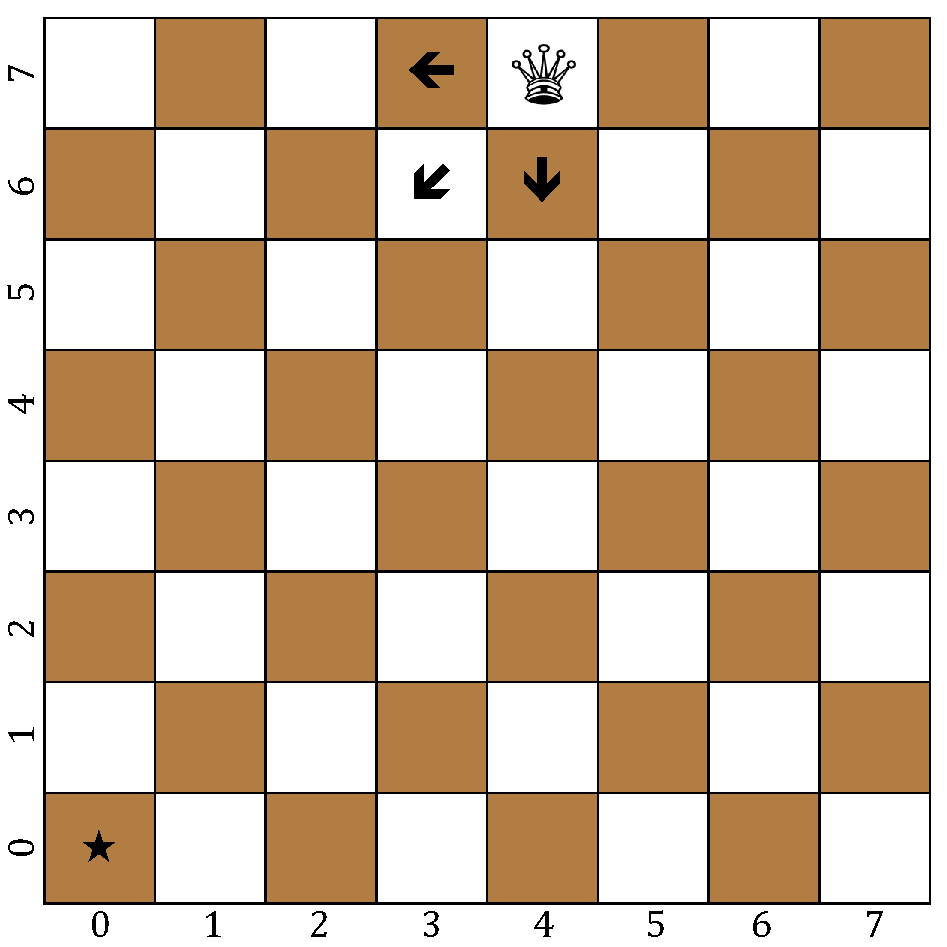
\includegraphics[height=2.5in]{figures/cornerqueen.pdf}
\caption{Cornering the Queen.\label{fig:cornerqueen}}
\end{center}
\end{figure}

On each turn, a player moves the Queen one or more squares in either the left, down, or diagonally down-left direction (unlike a standard chess Queen, in this game the queen may not move right, up or up-right).  As with the other games, the last player to make a legal move wins.  For this game, once the Queen reaches the bottom left square marked with the $\star$, there are no moves possible.  Hence, the player who moves the Queen onto the $\star$ wins the game.  We name the squares using the numbers on the sides of the chessboard with the column number first.  So, the Queen in the picture is on square \scheme|(4 7)|.

\resume{subexerciselist}
\item Identify all the starting squares for which the first played to move can win right away.  (Your answer should generalize to any size square chessboard.)
\item Suppose the Queen is on square \scheme|(2 1)| and it is your move.  Explain why there is no way you can avoid losing the game.
%\item If the Queen is on square \scheme|(5 6)| and it is your move, how should you move to guarantee you will win the game?
\item \greenstar Given the shown starting position (with the Queen at \scheme|(4 7)|, would you rather be the first or second player?
\item \goldstar Describe a strategy for winning the game (when possible).  Explain from which starting positions it is not possible to win (assuming the other player always makes the right move).
\item \goldstar Define a variant of Nim that is essentially the same as the ``Corner the Queen'' game.  (This game is known as ``Wythoff's Nim''.)
\end{subexerciselist}

Developing winning strategies for these types of games is similar to defining a recursive procedure that solves a problem.  We need to identify a base case from which it is obvious how to win, and a way to make progress fro	m a large input towards that base case.

}

\section{Summary}

By breaking problems down into simpler problems we can develop solutions to complex problems.  Many problems can be solved by combining instances of the same problem on simpler inputs.  When we define a procedure to solve a problem this way, it needs to have a predicate expression to determine when the base case has been reached, a consequent expression that provides the value for the base case, and an alternate expression that defines the solution to the given input as an expression using a solution to a smaller input.  

\groupcontent{
Our general recursive problem solving strategy is:
\begin{enumerate}
\item \bold{Be optimistic!}  Assume you can solve it.  
\item Think of the simplest version of the problem, something you can already solve.  This is the base case.
\item Consider how you would solve a big version of the problem by using the result for a slightly smaller version of the problem.  This is the recursive case.
\item Combine the base case and the recursive case to solve the problem.
\end{enumerate}
}

\sidequote{I'd rather be an optimist and a fool than a pessimist and right.}{Albert Einstein}\index{people}{Einstein, Albert}
For problems involving numbers, the base case is often when the input value is zero\cut{ (but not always, as we saw in the \scheme{find-maximum} value, where the base case is reached when the difference between two of the input values is zero)}.  The problem size is usually reduced is by subtracting \scheme|1| from one of the inputs. 

In the next chapter, we introduce more complex data structures.  For problems involving complex data, the same strategy will work but with different base cases and ways to shrink the problem size.

%%\cut{ % remove for copyright
\begin{center}
{\scalebox{0.50}{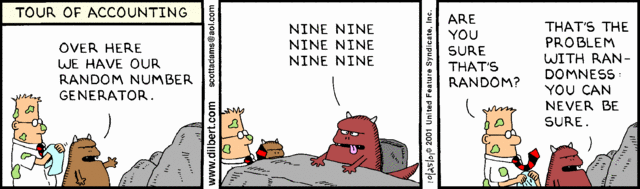
\includegraphics{images/dilbert.png}}} 
%http://www.dilbert.com/strips/comic/2001-10-25/
\cut{\vskip 1ex
\subcap{Producing good random numbers is an important and interesting problem, as is the question of determining whether a given sequence of numbers is random.  We consider it in Chapter~\ref{ch:alternatemodels}.}}
\end{center} % Need permission!
}
%%}

\end{schemeregion}
